\section{Results}

\subsection{Simulated Annealing}
This section lists some SA optimizations for comparison.

\subsubsection{Run 1} 
\label{sec:run_1}

\begin{tabular}{lr}
	Min: 			& 127030005662992 \\
	Max:			& 1636549083561452 \\
	Standard Deviation:	& 217723255965676\\
\end{tabular}

\begin{figure}[!h]
	\begin{center}
		\includegraphics[width=120mm]{images/saXX_exc}
               	\caption{SA muscle excitation patterns}
                \label{saXX_exc}
        \end{center}
\end{figure}

\pagebreak
\begin{figure}[!h]
	\begin{center}
		\includegraphics[width=120mm]{output/sa01/graph_all.pdf}
               	\caption{SA fitness over generations}
                \label{saXX_exc}
        \end{center}
\end{figure}

\pagebreak
\begin{figure}[!h]
	\begin{center}
		\includegraphics[width=120mm]{output/sa01/graph_70.pdf}
               	\caption{Same SA fitness over last 70 generations}
                \label{sa01_70_exc}
        \end{center}
\end{figure}

\pagebreak

\subsection{Genetic Algorithm with Mutation Only}

\subsubsection{GA Run 1}
\begin{tabular}{lr}
	Min: 			& 127156943557514  \\
	Max:			& 127354767955212  \\
	Standard Deviation:	& 35435274465.6039 \\
\end{tabular}

Parameters for ga:\\
\begin{tabular}{lr}
	POP\_SIZE:	& 10 \\
	ATTR\_SIZE:	& 96 \\
	GA\_LBOUND:	& -5.000 \\
	GA\_UBOUND:	& 100.00 \\
	GA\_DIFF\_SCALE: & 800.000 \\
	K\_MUT:		& 96 \\
	K\_SELECT:	& 1 \\
\end{tabular}

\begin{figure}[!h]
	\begin{center}
		\includegraphics[width=120mm]{output/ga01/graph.pdf}
               	\caption{GA fitness, uniform mutation only}
                \label{ga01_exc}
        \end{center}
\end{figure}

\pagebreak
\subsubsection{GA Run 2}
\begin{tabular}{lr}
	Min: 			& 126393050706189   \\
	Max:			& 126471924413236   \\
	Standard Deviation:	& 24842647883.601  \\
\end{tabular}


Parameters for ga:\\
\begin{tabular}{lr}
	POP\_SIZE:	& 10 \\
	ATTR\_SIZE:	& 96 \\
	GA\_LBOUND:	& -5.000 \\
	GA\_UBOUND:	& 100.00 \\
	GA\_DIFF\_SCALE: & 800.000 \\
	K\_MUT:		& 96 \\
	K\_SELECT:	& 1 \\
\end{tabular}

\begin{figure}[!h]
	\begin{center}
		\includegraphics[width=120mm]{output/ga02/graph.pdf}
               	\caption{Another GA fitness, uniform mutation only}
                \label{saXX_exc}
        \end{center}
\end{figure}

\pagebreak
\subsection{Genetic Algorithm with Uniform Mutation and Point Crossover}
\subsubsection{GA Run 3}
\begin{tabular}{lr}
	Min: 			& 126286311965193 \\
	Max:			& 126903624988318 \\
	Standard Deviation:	& 226416086588.11 \\
\end{tabular}

Parameters for ga:\\
\begin{tabular}{lr}
	POP\_SIZE:	& 10 \\
	ATTR\_SIZE:	& 96 \\
	GA\_LBOUND:	& -5.000 \\
	GA\_UBOUND:	& 100.00 \\
	GA\_DIFF\_SCALE: & 800.000 \\
	K\_MUT:		& 96 \\
	K\_SELECT:	& 1 \\
	K\_FLIP\_XOVER:	& 1 \\
\end{tabular}

\begin{figure}[!h]
	\begin{center}
		\includegraphics[width=120mm]{output/ga03/graph.pdf}
               	\caption{GA fitness, uniform mutation and one point flip crossover}
                \label{saXX_exc}
        \end{center}
\end{figure}


\subsection{Algorithm Comparison}
\begin{tabular}{llll}
Optimization	& Min			& Max			& Standard Deviation \\
SA		& 127030005662992 	& 1636549083561452	& 217723255965676 \\
GA Run 1	& 127156943557514	& 127354767955212	& 35435274465.6039 \\
GA Run 2	& 126393050706189	& 126471924413236	& 24842647883.601 \\
GA Run 3	& 126286311965193	& 126903624988318	& 226416086588.11 \\
\end{tabular}
